% @author: Jan Svacina
% @author: Jonathan Simmons

\documentclass{article}


\usepackage{fullpage}
\usepackage{url}

\usepackage{amssymb}
\usepackage{amsmath}

%\let\emptyset\emptyset
%\let\emptyset\varnothing

\usepackage[letterspace=150]{microtype}

%\usepackage{enumitem}
%\usepackage{flexisym} % https://tex.stackexchange.com/questions/36655/prime-in-text-mode
%\usepackage{commath}
%\usepackage{graphicx}
%\graphicspath{ {./} }

\let\oldemptyset\emptyset
\let\emptyset\varnothing

    \usepackage{listings}
\usepackage{color}

%\definecolor{codegreen}{rgb}{0,0.6,0}
%\definecolor{codegray}{rgb}{0.5,0.5,0.5}
%\definecolor{codepurple}{rgb}{0.58,0,0.82}
%\definecolor{backcolour}{rgb}{0.95,0.95,0.92}
%
%\lstdefinestyle{mystyle}{
%backgroundcolor=\color{backcolour},
%commentstyle=\color{codegreen},
%keywordstyle=\color{magenta},
%numberstyle=\tiny\color{codegray},
%stringstyle=\color{codepurple},
%basicstyle=\footnotesize,
%breakatwhitespace=false,
%breaklines=true,
%captionpos=b,
%keepspaces=true,
%%numbers=left,
%numbersep=5pt,
%showspaces=false,
%showstringspaces=false,
%showtabs=false,
%tabsize=2,
%%basicstyle=\lage
%}
%
%\lstset{style=mystyle}

% tell Latex to use no paragraph indentation, but leave some space between
% paragraphs
\setlength{\parindent}{0in}
\setlength{\parskip}{0.1in}

\usepackage{hyperref}
\hypersetup{
colorlinks=true,
linkcolor=blue,
filecolor=magenta,
urlcolor=blue,
}
\urlstyle{same}

\lstset{
language=C,                % choose the language of the code
%numbers=left,                   % where to put the line-numbers
%stepnumber=1,                   % the step between two line-numbers.
numbersep=5pt,                  % how far the line-numbers are from the code
backgroundcolor=\color{white},  % choose the background color. You must add \usepackage{color}
showspaces=false,               % show spaces adding particular underscores
showstringspaces=false,         % underline spaces within strings
showtabs=false,                 % show tabs within strings adding particular underscores
tabsize=2,                      % sets default tabsize to 2 spaces
captionpos=b,                   % sets the caption-position to bottom
breaklines=true,                % sets automatic line breaking
breakatwhitespace=true,         % sets if automatic breaks should only happen at whitespace
title=\lstname,                 % show the filename of files included with \lstinputlisting;
}


\usepackage{graphicx}
\graphicspath{ {./images/} }
\usepackage[final]{pdfpages}
%\usepackage{fullpage}
%\usepackage{url}
%\usepackage{hyperref}
%\usepackage{amssymb}
%\usepackage{amsmath}
%\usepackage[letterspace=150]{microtype}
%\usepackage{enumitem}
%\usepackage{graphicx}
%\graphicspath{ {./images/} }
%
%\hypersetup{
%colorlinks=true,
%linkcolor=blue,
%filecolor=magenta,
%urlcolor=blue,
%}
%\urlstyle{same}
%% tell Latex to use no paragraph indentation, but leave some space between
%% paragraphs
%\setlength{\parindent}{0in}
%\setlength{\parskip}{0.1in}
%\usepackage[final]{pdfpages}


\title{Iteration II}
\date{10/24/19}
\author{Jonathan Simmons, Jan Svacina}

\begin{document}

    \maketitle
    \section{Summary}
    \textbf{Problem Statement}\\
    Problem: Code clone tools are
    \begin{enumerate}
        \item dependent on a parser that parses the language
        \item dependent on a language specification that evolves
    \end{enumerate}
    Proposed solution:
    \begin{enumerate}
        \item Use classification based on deep learning
        \item Label each line of code as variable assignment, method call, etc
        \item Group code segments through deep learning
        \item Maximize interesting code snippets by maximizing entropy
    \end{enumerate}
    Benefits:\\
    - Building and running a model is faster than writing or running a parser

    Application:\\
    - Search for some patterns in classified code

    Benefits:\\
    - Increase semantic code clone detection efficiency by reducing the codebase to be analyzed \\
    - We pose that while running this learning model will take time t1 on a system S1 and running a semantic code clone detection algorithm on system S1 will take time t2 and that though the overall composite time cost is t1+ t2, eventually, as the model decreases the size of S1 and in turn t2$>$t3 , the new composite speed will be quicker: t1+t2$>$t1+t3.\\
    - (Or that there will exist a point in which running both this model and a given semantic code clone detection algorithm in tandem will be quicker than running just a semantic code clone detection algorithm.)

    \textbf{Proposed Approach Overview}
    \begin{enumerate}
        \item Classify code
        \item Find interesting parts of code
        \item Compare interesting parts of code by standard techniques
    \end{enumerate}

    \textbf{Theoretical Classifications for Lines of Code}
    \begin{itemize}
        \item Stereotypes lines of code
        \item Variable and method associations
    \end{itemize}
    We will weight stereotypes by how much they could impact entropy (e.g. method calls have more behavior and information than assigning to an integer)

    We will recognize those that we will call "Uninteresting Stereotypes":
    \begin{itemize}
        \item Import statements
        \item Printing
        \item Logging
        \item etc.
    \end{itemize}

    \textbf{Finding Interesting Code segments}\\
    Deriving interesting part out of code snippets, sanitize from the pool those segments which contain solely uninteresting segments (from the labeling).

    Segments, such as the following, that contain highly repetitive patterns that provide no meaningful semantics will be filtered out (low entropy):
    \begin{lstlisting}
    assignment::primitive
    assignment::primitive
    assignment::primitive
    assignment::primitive
    \end{lstlisting}
    \textbf{Problems to Address}\\
    \textit{How do we single out segments to determine their entropy and in turn interest value?}\\
    Greedy approach of moving the selection window up and down increasing height to get maximum entropy. If the maximum entropy was found previously at a smaller height, decrease.
    We let the algorithm find the boundary of the window by learning what is considered interesting with respect to our classifications and example code.

    We will then supply a standard semantic code clone detection software with this subset of code segments gathered from our deep learning model.

    \textbf{Current Status}
    \begin{itemize}
        \item A basic set of classifications for prototyping (single layer)
        \item A 4 layer sequential neural network (128 x 128 x 128 x 2). The input fires up to 128 neurons for a line length maximum of 128, based on token recognition.
        \item Benefit: Easy to produce network
        \item Down-side: Token based, recognition is based solely on largeness of dataset size
        \item 2 output neurons ((0.23, 0.77) -> %23 loop, %77 conditional)
        \item 4,000 auto generated loop / conditional statements for testing
    \end{itemize}

    \textbf{Current Progress Direction} \\
    Our v1 prototype classifications\\
    - Loop, Conditional\\
    Once v1 is verified, expand to v2\\
    - Loop, Conditional, Method Call, Assignment, Creation of new object, Termination, Switch, Case, Lambda, Inline\\
    Once v2 is verified, expand to v3\\
    - Convolution / filtering for Assignment::primitive, Assignment::object, Creation::new, Creation::method etc.\\

    \textbf{Future Work}\\
    The case of multiple, separate, interesting segments in a single method\\
    - Currently we search for the maximum possible entropy of one code segment per method. What if a method performs two distinct and low cohesion behaviors?\\
    Run the experiment and prove that there is some substantive speedup when running our model + traditional semantic code clone detection\\
    Tweak our classifications and weights for best results\\
    Train the model based on word associations rather than tokens\\
    - Experimentally we showed with predictable predicate names, accuracy dramatically increased.\\
    - Tokenize - lose language agnostic property\\
    - Word association - keep agnosticism, gain accuracy, reduce loss\\

    \section{References}
    This section shows
    \lstinputlisting[mathescape=true, escapechar=\%, language=python, caption=generate a code snippet that is conditional,
    captionpos=b]{snippets/gen-cond.py}

    \lstinputlisting[mathescape=true, escapechar=\%, language=python, caption=generate a random conditional,
    captionpos=b]{snippets/conditionals.py}

    \lstinputlisting[mathescape=true, escapechar=\%, language=python, caption=format the json files to code snippet vs. classification,
    captionpos=b]{snippets/creating-training.py}

    \lstinputlisting[mathescape=true, escapechar=\%, language=python, caption=imported libraries,
    captionpos=b]{snippets/imports.py}

    \lstinputlisting[mathescape=true, escapechar=\%, language=python, caption=generate random predicate,
    captionpos=b]{snippets/predicate.py}

    \lstinputlisting[mathescape=true, escapechar=\%, language=python, caption=reading the training and classification sets,
    captionpos=b]{snippets/reading.py}

    \lstinputlisting[mathescape=true, escapechar=\%, language=python, caption=creating and running the keras model training,
    captionpos=b]{snippets/running-model.py}

    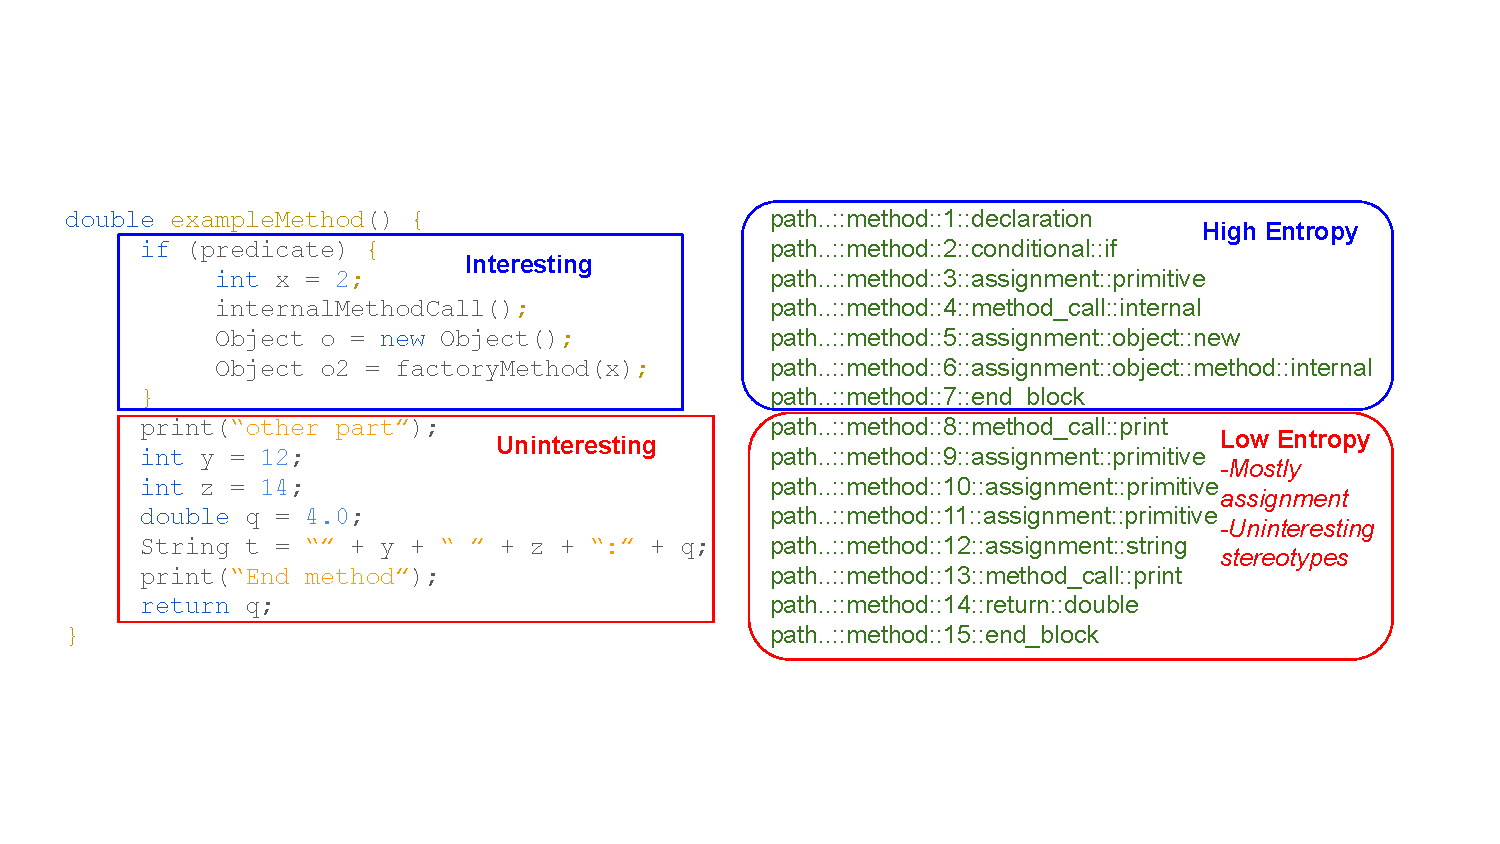
\includepdf[pages=-,pagecommand={},width=\textwidth]{images/01.pdf}

    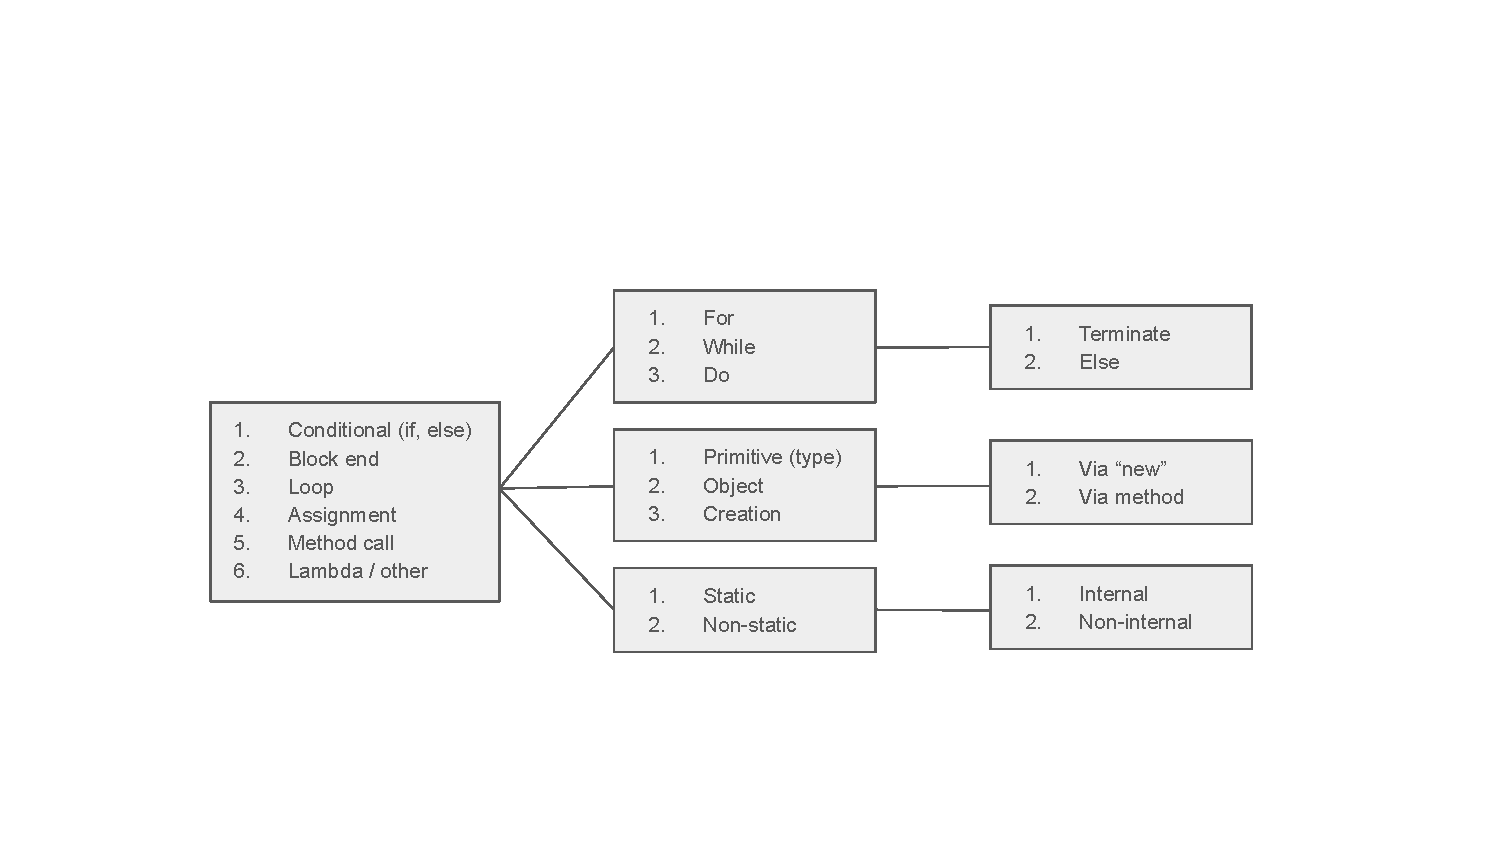
\includepdf[pages=-,pagecommand={},width=\textwidth]{images/02.pdf}

    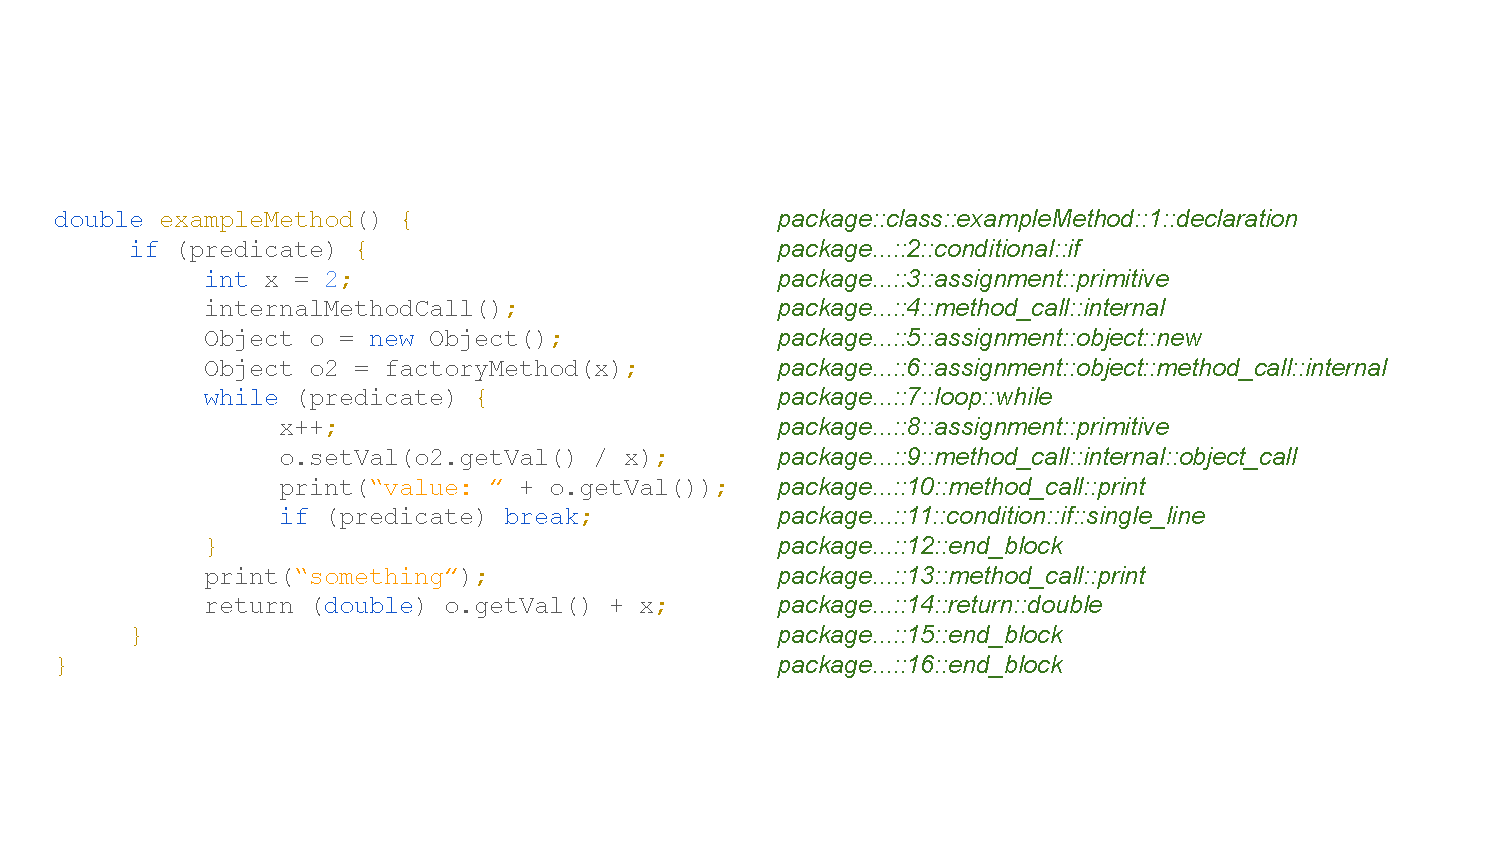
\includepdf[pages=-,pagecommand={},width=\textwidth]{images/03.pdf}


    \section{Worksheets}


    \subsection*{Jonathan Simmons}

    \begin{center}
        \begin{tabular}{||c c ||}
            \hline
            Number of tasks: &  \\
            \hline
            Number of commits: &  \\
            \hline
            Number of hours: &  \\
            \hline
        \end{tabular}
    \end{center}

    \subsection*{Jan Svacina}

    \begin{center}
        \begin{tabular}{||c c ||}
            \hline
            Number of tasks: &  \\
            \hline
            Number of commits: &  \\
            \hline
            Number of hours: &  \\
            \hline
        \end{tabular}
    \end{center}




\end{document}
